\documentclass[a0,landscape]{a0poster}

\usepackage{hyperref}
\bibliographystyle{plain}
%\usepackage{acl2014}
\newcommand{\newcite}[1]{\cite{#1}}   % ACL's newcite is not available in plain bib style, so just use cite1

\usepackage{multicol} % This is so we can have multiple columns of text side-by-side
\columnsep=100pt % This is the amount of white space between the columns in the poster
\columnseprule=3pt % This is the thickness of the black line between the columns in the poster

\usepackage[svgnames]{xcolor} % Specify colors by their 'svgnames', for a full list of all colors available see here: http://www.latextemplates.com/svgnames-colors

\usepackage{times} % Use the times font
%\usepackage{palatino} % Uncomment to use the Palatino font

\usepackage{graphicx} % Required for including images
\usepackage{booktabs} % Top and bottom rules for table
\usepackage[font=small,labelfont=bf]{caption} % Required for specifying captions to tables and figures
\usepackage{amsfonts, amsmath, amsthm, amssymb} % For math fonts, symbols and environments
\usepackage{wrapfig} % Allows wrapping text around tables and figures


%\usepackage{xspace}
%\usepackage{enumitem}
%\usepackage[small]{caption}
%\usepackage{longtable}

%\usepackage{soul}

\usepackage{algorithm}
\usepackage[noend]{algpseudocode}
%\usepackage{caption}
\usepackage{subcaption}
\usepackage{pdfpages}

\usepackage{tikz-dependency}

\newcommand{\eqnref}[1]{\eqref{eqn:#1}}

\usepackage[disable]{todonotes}   % insert [disable] to disable all notes
% Note that these macros accept optional arguments such as 
% [size=\small,bordercolor=red].
\newcommand{\Note}[4][]{\todo[author=#2,color=#3,fancyline,#1]{#4}}
\newcommand{\noteJH}[2][]{\Note[size=\small,#1]{JH}{blue!40}{#2}}
\newcommand{\noteJE}[2][]{\Note[size=\small,#1]{JE}{green!40}{#2}}   
\newcommand{\notewho}[3][]{\Note[size=\small,#1]{#2}{orange!40}{#3}}  % extra arg with miscellaneous author
\newcommand{\NoteJH}[2][]{\noteJH[inline,#1]{#2}}
\newcommand{\NoteJE}[2][]{\noteJE[inline,#1]{#2}}
\newcommand{\Notewho}[3][]{\notewho[inline,#1]{#2}{#3}}  % extra arg with miscellaneous author




\begin{document}

%----------------------------------------------------------------------------------------
%	POSTER HEADER 
%----------------------------------------------------------------------------------------

% The header is divided into three boxes:
% The first is 55% wide and houses the title, subtitle, names and university/organization
% The second is 25% wide and houses contact information
% The third is 19% wide and houses a logo for your university/organization or a photo of you
% The widths of these boxes can be easily edited to accommodate your content as you see fit
%
\begin{minipage}[b]{0.19\linewidth}
  \begin{flushleft}
    
\includegraphics[width=15cm]{lti_logo.png} % Logo or a photo of you, adjust its dimensions here
  \end{flushleft}
\end{minipage}
%
\begin{minipage}[b]{0.55\linewidth}
  \centering \veryHuge \color{NavyBlue} \textbf{Deriving Multi-Headed Planar Dependency Parses from Link Grammar Parses} 
 \color{Black} \\
  %\Huge\textit{An Exploration of Complexity}\\[1cm] % Subtitle
\begin{minipage}{0.4\linewidth}
  \begin{flushleft}
  \centering \huge \textbf{Juneki Hong}\\
  \centering \huge Carnegie Mellon University 
  \end{flushleft}
\end{minipage}
\begin{minipage}{0.4\linewidth}
  \begin{flushright}
  \centering \huge \textbf{Jason Eisner}\\
  \centering \huge Johns Hopkins University
  \end{flushright}
\end{minipage}
\end{minipage}
\begin{minipage}[b]{0.19\linewidth}
  \begin{flushright}
    
\includegraphics[width=10cm]{jhu_seal.png}
  \end{flushright}
\end{minipage}


\vspace{1cm} % A bit of extra whitespace between the header and poster content

%----------------------------------------------------------------------------------------

\begin{multicols}{4} % This is how many columns your poster will be broken into, a poster with many figures may benefit from less columns whereas a text-heavy poster benefits from more

\color{Navy} % Navy color for the summary


\section*{Summary}

\begin{itemize}
\item Multi-headed dependency corpora would allow for the development of richer syntactic formalisms. 
%However few exist, especially for the planar or projective case.
\item In order to produce projective multi-headed corpora, we consistently directionalize Link Grammar using Integer Linear Programming.
\item The resulting parses differ in style from CoNLL-style parses of the same sentences.
\end{itemize}
\color{DarkSlateGray} % DarkSlateGray color for the rest of the content

\vspace{-5mm}
\section*{Multi-Headed Dependency Parsing}
Relaxing single-headed constraints common in dependency parsing would allow for constructions such as Control, Relativization, and Conjunction.
%
\vspace{-5mm}
\subsection*{Control}
%
\begin{figure}[H]
  \centering
  %\begin{dependency}
  %  \begin{deptext}
  %    Jill \& likes \& to \& skip \\
  %  \end{deptext}
  %  \deproot[edge above, thick, hide label, edge unit distance = 1.5ex]{2}{}
  %  \depedge[edge above, thick, hide label]{2}{1}{}
  %  \depedge[edge below, ultra thick, hide label, edge style = {purple}, edge unit distance = 0.9ex]{4}{1}{}
  %  \depedge[edge above, thick, hide label]{2}{3}{}
  %  \depedge[edge above, thick, hide label]{3}{4}{}
  %\end{dependency}
  %\caption*{Jill is the subject of two verbs}
  \begin{dependency}
    \begin{deptext}
      Jill \& persuaded \& Jack \& to \& skip \\
    \end{deptext}
    \deproot[edge above, thick, hide label, edge unit distance = 1.5ex]{2}{}
    \depedge[edge above, thick, hide label]{2}{1}{}
    \depedge[edge above, thick, hide label]{2}{3}{}
    \depedge[edge above, thick, hide label]{3}{4}{}
    \depedge[edge above, thick, hide label]{4}{5}{}
    \depedge[edge below, ultra thick, hide label, edge style = {purple}, edge unit distance = 1.5ex]{5}{3}{}
    \depedge[edge below, ultra thick, hide label, edge style = {purple}, edge unit distance = 1.5ex]{2}{5}{}
  \end{dependency}
  \caption*{Jack is the object of one verb and the subject of another}
\end{figure}
%
\vspace{-5mm}
%
\subsection*{Relativization}
%
\begin{figure}[H]
  \centering
  \begin{dependency}
    \begin{deptext}
      The \& boy \& that \& Jill \& skipped \& with \& fell \& down \\
    \end{deptext}
    \deproot[edge above, thick, hide label, edge unit distance = 2ex]{7}{}
    \depedge[edge above, thick, hide label]{2}{1}{}
    \depedge[edge above, thick, hide label]{2}{3}{}
    \depedge[edge above, thick, hide label]{3}{5}{}
    \depedge[edge above, thick, hide label]{5}{4}{}
    \depedge[edge above, thick, hide label]{5}{6}{}
    \depedge[edge above, thick, hide label, edge unit distance = 1.4ex]{7}{2}{}
    \depedge[edge above, thick, hide label]{7}{8}{}
    \depedge[edge below, ultra thick, hide label, edge style = {purple}, edge unit distance = 1.0ex]{6}{2}{}
  \end{dependency}
  \caption*{The boy is the object of \textit{with} as well as the subject of \textit{fell}.}
\end{figure}
%
\vspace{-5mm}
%
\subsection*{Conjunction}
\begin{figure}[H]
  \centering
  \begin{dependency}
    \begin{deptext}
      Jack \& and \& Jill \& went \& up \& the \& hill \\
    \end{deptext}
    \deproot[edge above, thick, hide label, edge unit distance = 2ex]{4}{}
    \depedge[edge above, thick, hide label]{2}{1}{}
    \depedge[edge above, thick, hide label]{2}{3}{}
    \depedge[edge above, thick, hide label]{4}{2}{}
    \depedge[edge above, thick, hide label]{4}{5}{}
    \depedge[edge above, thick, hide label]{5}{7}{}
    \depedge[edge above, thick, hide label]{7}{6}{}
    \depedge[edge below, ultra thick, hide label, edge style = {purple}, edge unit distance = 1.3ex]{4}{1}{}
    \depedge[edge below, ultra thick, hide label, edge style = {purple}, edge unit distance = 1.5ex]{4}{3}{}
  \end{dependency}
  \caption*{Jack and Jill serve as the two arguments to \textit{and}, but are also subjects of \textit{went}.}
\end{figure}
%
\section*{Link Grammars}
\begin{itemize}
\item Grammar-based formalism for projective dependency parsing with undirected links. 
\item A label on the link describes the relationship between two words.
\item The original formalism and English Link Grammar was created by Davy Temperley, Daniel Sleator, and John Lafferty\cite{sleator-temperley-1991}.
\end{itemize}
%\vspace{-5mm}
\begin{figure}[H]
\centering
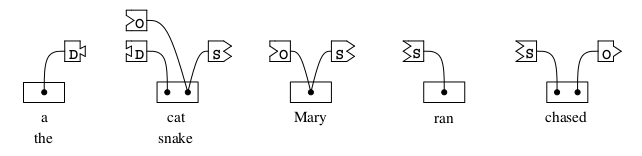
\includegraphics{linkgrammar_example1.png}
\caption*{Example visualization of a link grammar, taken from their original paper. Words have ``links'' that attach to others. These link attachments can either be optional or required.}
\end{figure}
\begin{figure}[H]
\centering

\includegraphics{linkgrammar_example2.png}
\caption*{A parse where all the link attachments have been satisfied. Link attachments must be projective. A parse cannot be completed until all words have a complete set of link attachments.}
\end{figure}
%\begin{figure}[H]
%\centering
%
\includegraphics{linkgrammar_example3.png}
%\caption*{Link attachments must be projective. A parse cannot be completed until all words have a complete set of link attachments.}
%\end{figure}

\section*{Integer Linear Programming}
\begin{itemize}
\item ILP is an optimization problem where the objective function and constraints are linear, while some or all of the variables are integers. 
\item In general, it's NP-Hard, but good solvers exist that often work well.
\item Our ILP is encoded as a ZIMPL program and solved with SCIP Optimization Suite\cite{Koch2004, achterberg2009scip}
\end{itemize}


\subsection*{Corpus Building Strategy}
\begin{itemize}
\item Start with corpus of link grammar parses to directionalize. 
\item Use ILP to find the minimum set of directionality assignments that satisfy constraints.
\end{itemize}
% such as acyclicity, connectedness, and directional consistency.

\subsection*{ILP Link Orientation Variables}
\begin{itemize}
\item[] For each sentence, for each edge $i,j$, where $i < j$
\begin{figure}[H]
  \centering
  \begin{dependency}[edge style={-}]
    \begin{deptext}
      . \& . \& . \& $i$ \& . \& . \& . \& $j$ \& . \& . \& . \\
    \end{deptext}
    \depedge[edge above, thick, edge unit distance = 1.1ex]{4}{8}{L}
  \end{dependency}
\end{figure}
\item[] Orientation of each link can be represented by variables that can either be oriented left or oriented right:
$$x_{ij}, x_{ji} \in \mathbb{Z} \geq 0$$
$$x_{ij} + x_{ji} = 1$$
\end{itemize}


\vspace{-2cm}
\subsection*{ILP Constraints}
\subsubsection*{Acyclicity}

\begin{itemize}
\item[] Given that node $u$ is the parent of $v$
\item[] $n_v$: length of the sentence containing node $v$
\item[] $d_v \in [0, n_v]$: depth of the node from the root of the sentence
\item[] We enforce that the depth of a child is greater than that of the parent:
\begin{align}
  (\forall_u)\; d_v + (1 + n_v) \cdot (1 - x_{uv}) & \geq 1+d_u
\end{align}
\end{itemize}

\subsubsection*{Connectedness}
To ensure that every word is reachable from a root, a word must have at least one parent. Together with acyclicity, this enforces connectedness.
\begin{align}
  \sum_u x_{uv} & \geq 1 
\end{align}


\subsubsection*{Consistency of Directionalized Links}
Links with same label type are encouraged to be oriented in the same way. We introduce variables to represent whether links with label $L$ are allowed to go left or right.
$$r_L, \ell_L \in \{0,1\}$$
We introduce slack variables $s_{ij}$ to allow some links to go in disallowed directions with a penalty.
\begin{itemize}  
\item[] $s_{ij} \in \mathbb{R} \geq 0$
\item[] $N_L$: number of link tokens with label $L$
\end{itemize}
\begin{align}\label{direction+slack}
  x_{ij} &\leq r_L + s_{ij} &
  x_{ji} &\leq \ell_L + s_{ij}
\end{align}
\begin{align}\label{eqn:obj}
  objective = \min \left( \sum_L r_L + \ell_L \right) \frac{N_L}{4} + \sum_{ij}s_{ij}
\end{align}







\section*{Data Sets}
Data Sets taken from:
\begin{itemize}
\item[] CoNLL 2007 Shared Task (English)
\item[] ACL 2013 Shared Task of Machine Translation (Russian)
\end{itemize}
\begin{figure}[H]
  \centering
  \begin{tabular}{|l|l|l|}
    \hline
    & Input Sentences & Output Connected Parses \\ \hline
    English  & 18,577        & 10,960               \\ \hline
    Russian & 18,577        & 4,913                \\ \hline
  \end{tabular}
\end{figure}

\section{Experiments and Results}

\begin{figure}
  \centering
  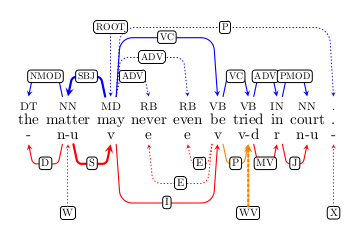
\includegraphics[width=0.6\linewidth]{example_parse.png}
  \caption*{Bottom half is from the CoNLL 2007 shared task. Top half is our directionalized link parse. Edges are shown as solid lines if they appear in both parses.  They are drawn more thickly if the directions do not match, and they are shown as dotted lines if they appear only in one parse and not in the other. Edges are highlighted in orange if the child has multiple parents.}
\end{figure}

\vspace{-5mm}
\begin{figure}[H]
  \centering
  \begin{dependency}
	\begin{deptext}
	  - \& n-u \& v \& e \& e \& v \& v-d \& r \& n-u \& - \\
	  the \& matter \& may \& never \& even \& be \& tried \& in \& court \& . \\
	  {\scriptsize DT} \& {\scriptsize NN} \& {\scriptsize MD} \& {\scriptsize RB} \& {\scriptsize RB} \& {\scriptsize VB} \& {\scriptsize VB} \& {\scriptsize IN} \& {\scriptsize NN} \& {\scriptsize .} \\
	\end{deptext}
	\deproot[edge below, thick, edge style = {blue}]{3}{\small ROOT}
	\depedge[edge above, thick, edge style = {red}]{2}{3}{S}
	\depedge[edge below, thick, edge style = {blue}]{3}{2}{\small SBJ}
	\depedge[edge below, thick, edge style = {blue}]{3}{4}{\small ADV}
	\depedge[edge below, thick, edge style = {blue}]{3}{5}{\small ADV}
	\depedge[edge above, thick, edge style = {red}]{3}{6}{I}
	\depedge[edge below, thick, edge style = {blue}]{3}{6}{\small VC}
	\depedge[edge below, thick, edge style = {blue}, edge unit distance =1.5ex]{3}{10}{\small P}
	\depedge[edge above, thick, edge style = {red}]{2}{1}{D}
	\depedge[edge below, thick, edge style = {blue}]{2}{1}{\small NMOD}
	\depedge[edge above, thick, edge style = {red}]{7}{8}{MV}
	\depedge[edge below, thick, edge style = {blue}]{7}{8}{\small ADV}
	\depedge[edge above, thick, edge style = {red}]{6}{7}{P}
	\depedge[edge below, thick, edge style = {blue}]{6}{7}{\small VC}
	\depedge[edge above, thick, edge style = {red}]{8}{9}{J}
	\depedge[edge below, thick, edge style = {blue}]{8}{9}{\small PMOD}
	\deproot[edge above, thick, edge style = {red}]{2}{W}
	\deproot[edge above, thick, edge style = {red}]{7}{WV}
	\deproot[edge above, thick, edge style = {red}]{10}{X}
	\depedge[edge above, thick, edge style = {red}]{6}{4}{E}
	\depedge[edge above, thick, edge style = {red}]{6}{5}{E}
  \end{dependency}

  \caption*{Bottom half from CoNLL 2007 shared task. Top half is our directionalized link parse.}
\end{figure}


\subsubsection*{Multiheadedness}
On the English data Set, the link data has 8\% additional edges over the CoNLL. (average about 2 multiheaded words per sentence)

\subsubsection*{CoNLL Matches}
\begin{itemize}
\item[] 52\% of links match CoNLL arcs
\item[] 57\% of CoNLL arcs match links
\end{itemize}

\subsubsection*{Directionality}
\begin{itemize}
\item[] 6.19\% of link types allowed both directions %($\frac{7}{113}$)
\item[] 2.07\% of link tokens required disallowed direction via slack %($\frac{4043}{195,000}$)
\end{itemize}

\subsection*{Stability of Results}
To see whether the recovered direction mapping might be unstable and sensitive to the input corpus, we compared results of increasing runs of sentences. 
\begin{figure}[H]
  \centering
  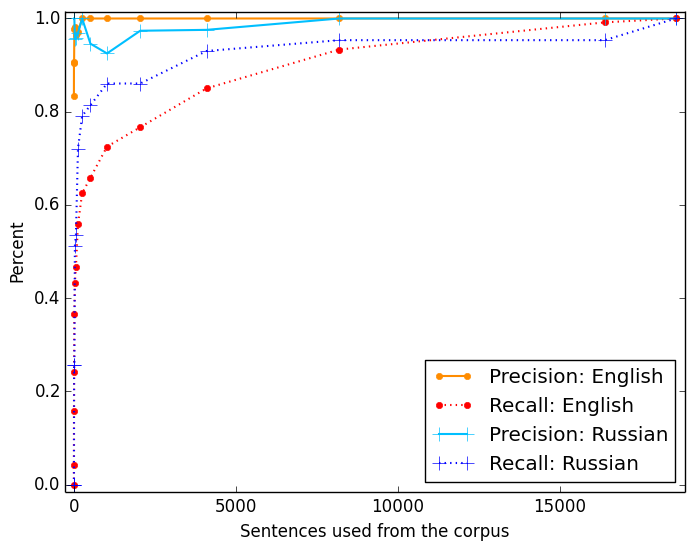
\includegraphics[width=0.6\linewidth]{precision_recall.png}
  \caption*{The direction mappings obtained on small datasets have high {\em precision} relative to the one obtained on the largest dataset.  Their {\em recall} grows as more link types are seen and directionalized.}\label{fig:convergence}
\end{figure}  
%Rapid convergence to the direction mapping obtained on the largest dataset.  

\vspace{-1cm}
\subsection*{Backwards Subject-Verb Links}
In our directionalized corpus subjects point to verbs instead of verbs pointing to subjects. This is due to a possible inconsistency of the Link Grammar discovered by our method.
\begin{itemize}
\item Link Grammar seems to be inconsistent about whether the auxiliary verb or the main verb is the head of a clause. 
\item Governing verb links to either auxilliary or main, depending on the clause type, but governing verbs usually link to subject when there is one. This makes subject a consistent choice to make head of a clause. To fix, we can edit the link grammar, link parses, or the ILP. 
\end{itemize}
%----------------------------------------------------------------------------------------
%	CONCLUSIONS
%----------------------------------------------------------------------------------------
\color{SaddleBrown} % SaddleBrown color for the conclusions to make them stand out
\vspace{-1cm}
\section*{Conclusions}
\begin{itemize}
\item Link Grammar parses can be oriented into connected DAGs
\item A new corpus for building multi-headed dependency parsers
\item ILP can be used to help annotate missing data in corpora. 
\end{itemize}


\color{DarkSlateGray} % Set the color back to DarkSlateGray for the rest of the content

%----------------------------------------------------------------------------------------
%	REFERENCES
%----------------------------------------------------------------------------------------

%\nocite{*} % Print all references regardless of whether they were cited in the poster or not
\begin{bibliography}{LinksToDAG_final}

\end{bibliography}

%----------------------------------------------------------------------------------------
%	ACKNOWLEDGEMENTS
%----------------------------------------------------------------------------------------

\subsubsection*{Acknowledgements}
This material is based upon work supported by the National Science Foundation under Grant No. 1423276.  The work was mainly conducted while the first author was at Johns Hopkins University.


%----------------------------------------------------------------------------------------

\end{multicols}
\end{document}
